En esta sección esperamos poder brindar una breve introducción a los temas que son relevantes para el desarrollo y la implementación de este proyecto. La dividiremos en tres partes: qué dataset elegimos y por qué; brindaremos una breve explicación que busca proveer al lector de las herramientas para poder interpretar la implementación; finalmente, explicaremos porque la aplicación de SIMD resulta pertinente a este problema.

\subsection{El dataset: MNIST}

El dataset MNIST\footnote{\url{http://yann.lecun.com/exdb/mnist/}} está compuesto por imágenes de dígitos manuscritos del 0 al 9, con una resolución de $28\times 28$ píxeles. A su vez, ya viene dividido en un training set de 60000 ejemplos (en particular, nosotros solo usamos 50000), y un test set de 10000.

Es un dataset que, por su simplicidad, está pensado para ser usado como un primer benchmark rápido para modelos, pudiendo abstraerse de las complicaciones inherentes al preprocesamiento de datos. 

En vista de que el objetivo central que se persigue es el de conseguir una optimización desde el punto de vista del tiempo de ejecución de las operaciones básicas, y no de la precisión del modelo (es decir, no nos interesa una red particularmente compleja), encontramos que este dataset se ajusta bien a nuestras necesidades: es lo bastante chico como para poder manejarlo con el hardware del que disponemos, pero no tanto como para no permitirnos hacer un análisis interesante. En este sentido, un dataset más complicado no nos aportaría nada.

\subsection{Redes Neuronales Artificiales}

No es la idea de esta sección brindar una introducción al amplio mundo de las RNAs. Nuestro objetivo es meramente dar definiciones mínimas y algoritmos necesarios (sin ninguna justificación teórica) para facilitar la interpretación del código. Para una explicación más profunda existe una basta bibliografía. En particular, este trabajo está fuertemente influenciado por el siguiente libro online: \url{http://neuralnetworksanddeeplearning.com/}.

\subsubsection{Definiciones}

Una RN es uno de los tantos modelos encuadrados dentro del paradigma del aprendizaje supervisado\footnote{\url{https://en.wikipedia.org/wiki/Supervised_learning}}. El elemento fundamental de las redes neuronales son las \emph{neuronas}. Una neurona computa una función con múltiples inputs y un output (todos números reales). La imagen (\ref{fig:neurona}) ilustra la estructura general de una neurona.

La función que ejecuta la neurona tiene dos partes. Primero una lineal (también llamada \emph{transfer function}), en la cual se multiplica a cada uno de los inputs $x_i$ por un cierto peso $w_i$, y posteriormente se los suma. En la suma suele participar un término independiente (llamado \emph{bias}), $b$. Es decir,

$$z = \sum w_i x_i + b$$

Luego, se le aplica a $z$ la llamada \emph{función de activación}, que nos dará el output de la neurona. Dicha función puede ser cualquiera que vaya de los reales a los reales, aunque típicamente se escogen ciertas funciones no lineales (se puede probar fácilmente que usar una función lineal no agrega mayor capacidad para aproximar funciones). En particular, para este trabajo usaremos como función de activación la función sigmoidea definida como sigue:

$$\sigma(z) = \frac{1}{1 + e^{-z}}$$

\begin{figure}[H]
  \begin{center}  
    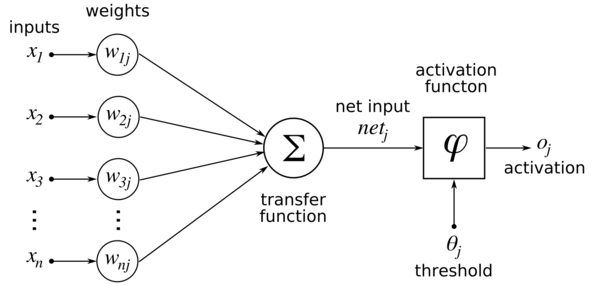
\includegraphics[width=0.8\linewidth]{imgs/neuron.png}
  \end{center}
  \caption{Estructura general de una neurona. }
  \label{fig:neurona}
\end{figure}

En general, una red neuronal va a consistir de muchas neuronas interconectadas (es decir que el output de una se vuelve el input de otra). Esto puede hacerse con diversas arquitecturas. En particular, nosotros usamos una de las más básicas que es la de Feedforward Neural Network. Esta es una arquitectura por capas o layers (donde cada capa es un conjunto de neuronas que no están interconectadas entre sí), en la cual el output de cada neurona de una capa alimenta al input de todas las neuronas de la capa siguiente (\emph{full connected}). En la siguiente imagen se ilustra esta arquitectura

\begin{figure}[H]
  \begin{center}  
    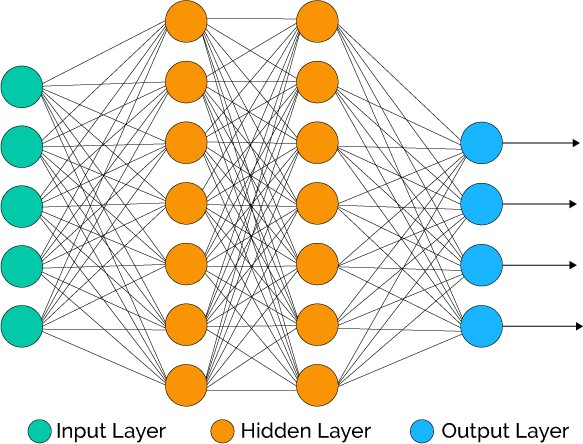
\includegraphics[width=0.7\linewidth]{imgs/multilayer_net.jpg}
  \end{center}
  \caption{Estructura general de una feedforward neural network}
  \label{fig:general_net}
\end{figure}

Puede verse que se diferencian tres tipos de capas: input layers, hidden layers y output layers. La primera y la última son bastante autoexplicativas; las capas ocultas (hidden) reciben ese nombre por el hecho de que los cómputos que realizan no son visibles por el usuario de la red, en contraposición con los inputs y los outputs que sí son ``visibles''. A una red como la de la imagen se la llama 3-layer neural network (no se cuenta la capa de input).

Por cuestiones que comentaremos en la sección siguiente, es conveniente adaptar una notación matricial para trabajar con los parámetros (pesos y \emph{biases} de las neuronas). Notaremos $w^l_{ij}$ como el peso correspondiente al input $j$-ésimo de la $i$-ésima neurona en la capa $l$. Similarmente $b^l_i$ será el bias correspondiente a la neurona $i$-ésima de la capa $l$.

Entonces, podemos definir las matrices $W^l$ tales que $(W^l)_{ij} = w^l_{ij}$, y los vectores $b^l$ tales que $(b^l)_i = b^l_i$ (no nos volvemos a referir a los valores individuales, así que los paréntesis no se usan más).

Las ecuaciones vistas antes para el cálculo del output de una neurona pueden generalizarse para el output de una capa de la siguiente manera:

$$z^l = W^l a^{l-1} + b^l$$
$$a^l = \sigma (z^l)$$

donde $1\leq l\leq L$, y definimos $a_0 = x$, con $x$ el input de la red. $\sigma$ en este caso es una función sobre un vector o una matriz y se aplica en forma \emph{element-wise}. Algo que puede generar confusión es que $x$ (y por lo tanto las subsecuentes $a^l$) puede ser tanto un vector como una matriz, de acuerdo a si hay uno o muchos inputs (cada input es un vector columna) tratando de computarse en simultáneo. Como usamos $mini-batches$ para entrenar, siempre será una matriz durante la fase de entrenamiento.

\subsubsection{Entrenamiento}

Pasemos ahora a la parte más importante, que es el algoritmo de entrenamiento de la red. Ante todo es importante entender que lo que queremos aprender son los parámetros $W^l$ y $b^l$. Además, es necesario definir una función de costo: es decir, una función que nos indique cuán ``lejos'' están las predicciones de las etiquetas verdaderas. Luego, el objetivo del entrenamiento será seleccionar los parámetros $W^l$ y $b^l$ que minimicen esta función.

Usaremos como función de costo el Error Cuadrático Medio (ECM)

$$C(W, b) = \frac{1}{2n}\sum_{x}{||y(x) - a||^2}$$

donde $w$ y $b$ son todos los parámetros de nuestra red, $y(x)$ es el output de la red para el input x, $a$ es el target verdadero para el input $x$, y $n$ es la cantidad de casos de entrenamiento.

La heurística de optimización usada es Gradient Descent\footnote{\url{https://en.wikipedia.org/wiki/Gradient_descent}}\footnote{En realidad, más correctamente usamos Stochastic Gradient Descent. Esto significa que en lugar de usar toda la data de entrenamiento antes de actualizar los parámetros, usamos pequeñas porciones  (\emph{mini-batches}) sampleadas aleatoriamente, lo que permite una mayor velocidad de convergencia. Debido a que es una técnica estándar del área decidimos aplicarla.}, por lo que en cada epoch ajustaremos los parámetros de la siguiente forma:

$$W^l_{ij} := W^l_{ij} - \eta \frac{\partial C}{\partial W^l_{ij}}$$
$$b^l_i := b^l_i - \eta \frac{\partial C}{\partial b^l_i}$$

donde $\eta$ es el \emph{learning rate} que determina cuánto queremos modificar nuestros parámetros en una iteración, y $\frac{\partial C}{\partial v}$ es la derivada parcial de $C$ respecto del parámetro $v$.

La pregunta que queda entonces es cómo calculamos las derivadas parciales. Para esto se utiliza un algoritmo conocido como \emph{backpropagation}. Recibe este nombre en contraposición al \emph{forward-propagation}, que es la pasada que se realiza sobre la red para calcular el output. Es decir que ahora querremos atravesar la red en sentido opuesto para calcular las derivadas parciales.

Nuevamente, no es la intención dar un \emph{insight} teórico sobre los algoritmos. Nos limitaremos a presentar el mismo, una justificación puede encontrarse en el libro citado arriba.

Para una L-layer neural network (recordar que con la input layer en rigor son L+1 layers), queremos calcular las matrices $\nabla W^l = \frac{\partial C}{\partial W^l}$, y los vectores $\nabla b^l = \frac{\partial C}{\partial b^l}$. Notar que estamos cometiendo un abuso de notación donde la derivada parcial respecto a una matriz (o un vector) es la matriz (o vector) que tiene las derivadas respecto de cada una de las componentes originales.

\begin{algorithm}
\caption{Backpropagation}\label{euclid}
\begin{algorithmic}[1]
\Procedure{backpropagation}{$Ws, bs, X, y$}
  \State $a^0 := X$
  \Comment Comienza pasada forward
  \For {$l \gets 1..\dots L$}
    \State $z^l := W^l a^{l-1} + b^l$
    \State $a^l := \sigma(z^l)$
  \EndFor 
  \State $\delta^{L} := (a^{L} - y)\odot \sigma^\prime(z^{L})$
  \Comment Comienza pasada backward
  \State $\nabla b^L := \delta^{l}$
  \State $\nabla W^L := \delta^l a^{(l-1)T}$
  \For {$l \gets (L-1)\dots1$}
    \State $\delta^{l} := ((W^{l+1})^T \delta^{l+1}) \odot \sigma^\prime(z^{l})$
    \State $\nabla b^l := \delta^{l}$
    \State $\nabla W^l := \delta^l a^{(l-1)T}$
  \EndFor
\EndProcedure
\end{algorithmic}
\end{algorithm} 

\subsection{Vectorización y Redes Neuronales}

En la sección anterior dimos definiciones y algoritmos en términos de matrices y vectores, lo cual puede resultar un poco más engorroso que si hiciéramos los cómputos de cada componente individualmente. 

La razón por la cual se decide hacer esto es una cuestión de performance: vectorizar permite explotar el paralelismo que dan las operaciones SIMD del procesador (o de una GPU en el caso más usado).

La naturaleza intrínsecamente vectorial de las redes neuronales fue lo que nos llevó a querer plantearnos este trabajo.